% begin module higher-derivatives-ex6
\begin{frame}
\begin{example}
If $f(x) = x^3-x$, find $f''(x)$.
\begin{columns}[c]
\column{.37\textwidth}
\psset{xunit=1.2cm, yunit=1.2cm}
\begin{pspicture}(-2,-2)(2,2)
\tiny
\fcAxesStandard{-2}{-2}{1.85}{2}
\fcLabelXOne
\fcLabelYOne
\uncover<8->{
%Function formula: 6 (x)
\psplot[linecolor=green, plotpoints=1000]{-0.333333333}{0.333333333}{x 6 mul }
\rput[br](-0.4,-2){$f''(x)$}
}
\uncover<2->{
%Function formula: 3 ((x)^{2})-1
\psplot[linecolor=blue, plotpoints=1000]{-1}{1}{-1 x 2 exp 3 mul add }
\rput[r](-1, 1){$f'(x)$}
}
%Function formula: - (x)+(x)^{3}
\psplot[linecolor=red, plotpoints=1000]{-1.521379707}{1.521379707}{x 3 exp x -1 mul add }
\rput[bl](1.2, 0.1){$f(x)$}
\end{pspicture}
%\ \only<handout:0| 1>{%
%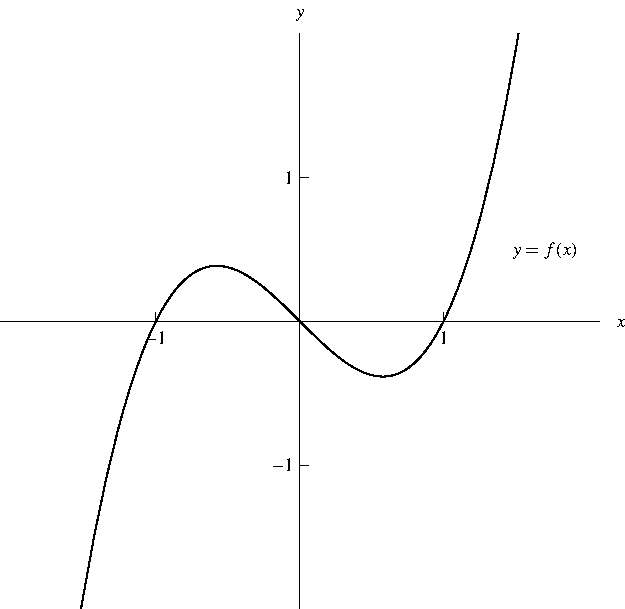
\includegraphics[height=4.5cm]{derivatives/pictures/03-02-ex6a.pdf}%
%}%
%\only<handout:0| 2-7>{%
%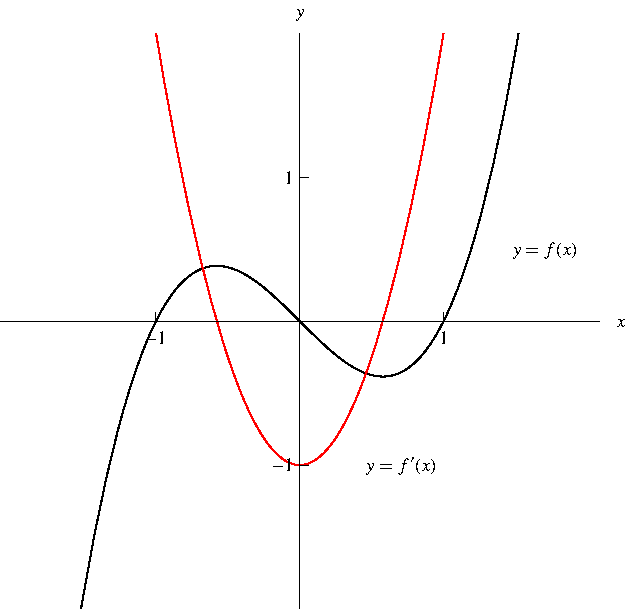
\includegraphics[height=4.5cm]{derivatives/pictures/03-02-ex6b.pdf}%
%}%
%\only<8->{%
%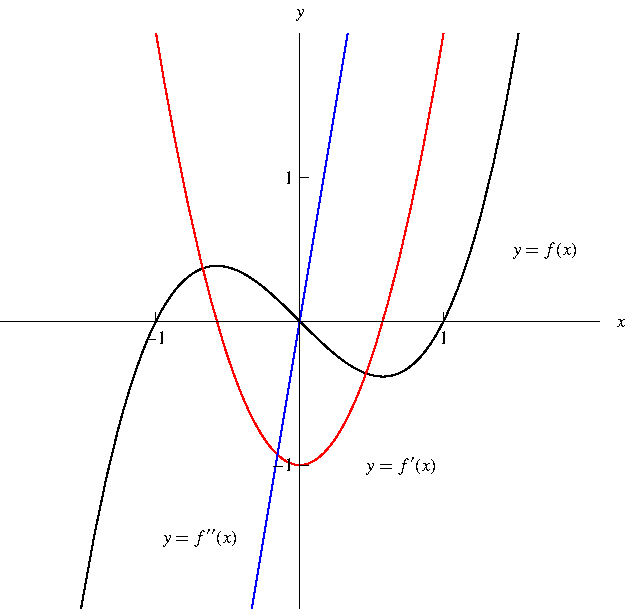
\includegraphics[height=4.5cm]{derivatives/pictures/03-02-ex6c.pdf}%
%}%

\column{.63\textwidth}
\uncover<2->{%
In a previous exercise we found that the first derivative is $f'(\alertNoH{4,5}{x}) = 3{\alertNoH{4,5}{x}}^2 - 1$.
}%
\abovedisplayskip=0pt
\belowdisplayskip=0pt
$
\begin{array}{@{}r@{}c@{}l}
\uncover<3->{f''(x)} & \uncover<3->{ = }  & \displaystyle \uncover<3->{\lim_{h\rightarrow 0}\frac{f'(\alertNoH{4}{x+h})-f'(\alertNoH{5}{x})}{h}}\\%
& \uncover<4->{ = }  & \displaystyle \uncover<4->{ \lim_{h \rightarrow 0} \frac{ \alertNoH{6}{3(\alertNoH{4}{ x+h})^2} -1 \alertNoH{7}{-\left(3 {\alertNoH{5}{x}}^2 -1\right)}}{h}}\\%
& \uncover<6->{ = }  & \displaystyle \uncover<6->{\lim_{h \rightarrow 0} \frac{ \alertNoH{6}{ \fcCancel{8}{3 x^2} + 6xh + 3h^2} -\fcCancel{8}{1} \alertNoH{7}{- \fcCancel{8}{3x^2} +\fcCancel{8}{1}}}{h}}\\%
& \uncover<8->{ = }  & \displaystyle \uncover<8->{\lim_{h \rightarrow 0}\frac{6x\alertNoH{9}{h} + 3{\alertNoH{9}{h}}^2}{h}}\\%
& \uncover<9->{ = }  & \displaystyle \uncover<9->{\lim_{h \rightarrow 0}\frac{\fcCancel{10}{\alertNoH{9}{h}}(6x + 3h)}{\fcCancel{10}{h}}}\\%
& \uncover<10->{ = }  & \displaystyle \uncover<10->{\alertNoH{11}{ \lim_{h \rightarrow 0}} ( 6x +\alertNoH{11}{ 3h} )}\uncover<11->{ = 6x}%
\end{array}
$
\end{columns}
\end{example}
\end{frame}
% end module higher-derivatives-ex6
